% ARQUIVO ÚNICO: as referências já estão dentro deste arquivo.
% No Overleaf, basta este arquivo (e, se quiser, figuras/blocos.png e figuras/pertinencias.png).
\begin{filecontents*}[overwrite]{refs.bib}
% Confira cada entrada no PDF/site do artigo antes de submeter. Entradas com TODO precisam ser completadas.

@inproceedings{chen2019,
  author    = {Chen, Tongfei and Navr{\'a}til, Ji{\v{r}}{\'\i} and Iyengar, Vijay and Shanmugam, Karthikeyan},
  title     = {Confidence Scoring Using Whitebox Meta-models with Linear Classifier Probes},
  booktitle = {Proceedings of the 22nd International Conference on Artificial Intelligence and Statistics (AISTATS)},
  series    = {Proceedings of Machine Learning Research},
  volume    = {89},
  pages     = {1467--1475},
  publisher = {PMLR},
  year      = {2019}
}

@inproceedings{corbiere2019,
  author    = {Corbi{\`e}re, Charles and Thome, Nicolas and Bar-Hen, Avner and Cord, Matthieu and P{\'e}rez, Patrick},
  title     = {Addressing Failure Prediction by Learning Model Confidence},
  booktitle = {Advances in Neural Information Processing Systems (NeurIPS)},
  year      = {2019}
}

@inproceedings{hendrycks2017,
  author    = {Hendrycks, Dan and Gimpel, Kevin},
  title     = {A Baseline for Detecting Misclassified and Out-of-Distribution Examples in Neural Networks},
  booktitle = {International Conference on Learning Representations (ICLR)},
  year      = {2017}
}

@inproceedings{gal2016,
  author    = {Gal, Yarin and Ghahramani, Zoubin},
  title     = {Dropout as a {B}ayesian Approximation: Representing Model Uncertainty in Deep Learning},
  booktitle = {International Conference on Machine Learning (ICML)},
  year      = {2016}
}

@inproceedings{lee2018,
  author    = {Lee, Kimin and Lee, Kibok and Lee, Honglak and Shin, Jinwoo},
  title     = {A Simple Unified Framework for Detecting Out-of-Distribution Samples and Adversarial Attacks},
  booktitle = {Advances in Neural Information Processing Systems (NeurIPS)},
  year      = {2018}
}

@article{papernot2018,
  author  = {Papernot, Nicolas and McDaniel, Patrick},
  title   = {Deep k-Nearest Neighbors: Towards Confident, Interpretable and Robust Deep Learning},
  journal = {arXiv preprint arXiv:1803.04765},
  year    = {2018}
}

@article{wangmendel1992,
  author  = {Wang, Li-Xin and Mendel, Jerry M.},
  title   = {Generating Fuzzy Rules by Learning from Examples},
  journal = {IEEE Transactions on Systems, Man, and Cybernetics},
  volume  = {22},
  number  = {6},
  pages   = {1414--1427},
  year    = {1992}
}

@article{takagi1985,
  author  = {Takagi, Tomohiro and Sugeno, Michio},
  title   = {Fuzzy Identification of Systems and Its Applications to Modeling and Control},
  journal = {IEEE Transactions on Systems, Man, and Cybernetics},
  volume  = {SMC-15},
  number  = {1},
  pages   = {116--132},
  year    = {1985}
}

@article{tschandl2018,
  author  = {Tschandl, Philipp and Rosendahl, Cliff and Kittler, Harald},
  title   = {The {HAM10000} Dataset, a Large Collection of Multi-Source Dermatoscopic Images of Common Pigmented Skin Lesions},
  journal = {Scientific Data},
  volume  = {5},
  pages   = {180161},
  year    = {2018}
}

@inproceedings{font2025,
  author    = {Font, Miguel N. and Jorro-Aragoneses, Jos{\'e} L. and Ala{\'\i}z, Carlos M.},
  title     = {A Framework for Uncertainty Quantification Based on Nearest Neighbors Across Layers},
  booktitle = {Artificial Neural Networks and Machine Learning -- ICANN 2025},
  series    = {Lecture Notes in Computer Science},
  volume    = {16068},
  pages     = {379--390},
  publisher = {Springer},
  year      = {2026},
  doi       = {10.1007/978-3-032-04558-4_30}
}

@inproceedings{gorbett2022,
  author    = {Gorbett, Matt and Blanchard, Nathaniel},
  title     = {Utilizing Network Features to Detect Erroneous Inputs},
  booktitle = {Proceedings of the IEEE/CVF Winter Conference on Applications of Computer Vision (WACV) Workshops},
  pages     = {34--43},
  year      = {2022}
}

@inproceedings{jaeger2023,
  author    = {Jaeger, Paul F. and L{\"u}th, Carsten T. and Klein, Lukas and Bungert, Till J.},
  title     = {A Call to Reflect on Evaluation Practices for Failure Detection in Image Classification},
  booktitle = {International Conference on Learning Representations (ICLR)},
  year      = {2023}
}

@inproceedings{guo2017,
  author    = {Guo, Chuan and Pleiss, Geoff and Sun, Yu and Weinberger, Kilian Q.},
  title     = {On Calibration of Modern Neural Networks},
  booktitle = {International Conference on Machine Learning (ICML)},
  year      = {2017}
}

@inproceedings{lakshminarayanan2017,
  author    = {Lakshminarayanan, Balaji and Pritzel, Alexander and Blundell, Charles},
  title     = {Simple and Scalable Predictive Uncertainty Estimation Using Deep Ensembles},
  booktitle = {Advances in Neural Information Processing Systems (NeurIPS)},
  year      = {2017}
}

@article{alain2016,
  author  = {Alain, Guillaume and Bengio, Yoshua},
  title   = {Understanding Intermediate Layers Using Linear Classifier Probes},
  journal = {arXiv preprint arXiv:1610.01644},
  year    = {2016}
}

@inproceedings{baldock2021,
  author    = {Baldock, Robert J. N. and Maennel, Hartmut and Neyshabur, Behnam},
  title     = {Deep Learning Through the Lens of Example Difficulty},
  booktitle = {Advances in Neural Information Processing Systems (NeurIPS)},
  year      = {2021}
}

@inproceedings{peterson2019,
  author    = {Peterson, Joshua C. and Battleday, Ruairidh M. and Griffiths, Thomas L. and Russakovsky, Olga},
  title     = {Human Uncertainty Makes Classification More Robust},
  booktitle = {Proceedings of the IEEE/CVF International Conference on Computer Vision (ICCV)},
  year      = {2019}
}

% TODO: conferir volume e páginas no site da IEEE
@article{aghaeipoor2023,
  author  = {Aghaeipoor, Fatemeh and Sabokrou, Mohammad and Fern{\'a}ndez, Alberto},
  title   = {Fuzzy Rule-Based Explainer Systems for Deep Neural Networks: From Local Explainability to Global Understanding},
  journal = {IEEE Transactions on Fuzzy Systems},
  year    = {2023}
}

@article{barna2026,
  author  = {Barna, Cornel and Petcut, Flavius-Maxim and Petcut-Lasc, Anca-Adriana},
  title   = {Reducing Image Classification Errors in Convolutional Neural Networks Through a Fuzzy--Possibilistic Abstention Mechanism},
  journal = {Applied Sciences},
  volume  = {16},
  number  = {21},
  pages   = {10568},
  year    = {2026}
}

% TODO: conferir volume e páginas no site da IEEE
@article{denoeux2023,
  author  = {Den{\oe}ux, Thierry},
  title   = {Quantifying Prediction Uncertainty in Regression Using Random Fuzzy Sets: The {ENNreg} Model},
  journal = {IEEE Transactions on Fuzzy Systems},
  year    = {2023}
}

@article{msaddi2026,
  author  = {Msaddi, Saleh and Kumbasar, Tufan},
  title   = {An Alliance for Uncertainty Quantification: Type-2 Fuzzy Logic Systems With Conformal Prediction},
  journal = {IEEE Transactions on Emerging Topics in Computational Intelligence},
  volume  = {10},
  number  = {2},
  pages   = {2022--2032},
  year    = {2026},
  doi     = {10.1109/TETCI.2025.3647649}
}


@inproceedings{wei2022,
  author    = {Jiaheng Wei and Zhaowei Zhu and Hao Cheng and Tongliang Liu and Gang Niu and Yang Liu},
  title     = {Learning with Noisy Labels Revisited: A Study Using Real-World Human Annotations},
  booktitle = {International Conference on Learning Representations (ICLR)},
  year      = {2022}
}

@inproceedings{song2019,
  author    = {Hwanjun Song and Minseok Kim and Jae-Gil Lee},
  title     = {{SELFIE}: Refurbishing Unclean Samples for Robust Deep Learning},
  booktitle = {International Conference on Machine Learning (ICML)},
  pages     = {5907--5915},
  year      = {2019}
}

@article{zhu2022,
  author  = {Chuang Zhu and Wenkai Chen and Ting Peng and Ying Wang and Mulan Jin},
  title   = {Hard Sample Aware Noise Robust Learning for Histopathology Image Classification},
  journal = {IEEE Transactions on Medical Imaging},
  volume  = {41},
  number  = {4},
  pages   = {881--894},
  year    = {2022}
}

@techreport{krizhevsky2009,
  author      = {Alex Krizhevsky},
  title       = {Learning Multiple Layers of Features from Tiny Images},
  institution = {University of Toronto},
  year        = {2009}
}

@inproceedings{he2016,
  author    = {Kaiming He and Xiangyu Zhang and Shaoqing Ren and Jian Sun},
  title     = {Deep Residual Learning for Image Recognition},
  booktitle = {IEEE Conference on Computer Vision and Pattern Recognition (CVPR)},
  pages     = {770--778},
  year      = {2016}
}

@inproceedings{simonyan2015,
  author    = {Karen Simonyan and Andrew Zisserman},
  title     = {Very Deep Convolutional Networks for Large-Scale Image Recognition},
  booktitle = {International Conference on Learning Representations (ICLR)},
  year      = {2015}
}

@inproceedings{sandler2018,
  author    = {Mark Sandler and Andrew Howard and Menglong Zhu and Andrey Zhmoginov and Liang-Chieh Chen},
  title     = {{MobileNetV2}: Inverted Residuals and Linear Bottlenecks},
  booktitle = {IEEE Conference on Computer Vision and Pattern Recognition (CVPR)},
  pages     = {4510--4520},
  year      = {2018}
}

@inproceedings{tan2019,
  author    = {Mingxing Tan and Quoc V. Le},
  title     = {{EfficientNet}: Rethinking Model Scaling for Convolutional Neural Networks},
  booktitle = {International Conference on Machine Learning (ICML)},
  pages     = {6105--6114},
  year      = {2019}
}

@inproceedings{dosovitskiy2021,
  author    = {Alexey Dosovitskiy and Lucas Beyer and Alexander Kolesnikov and Dirk Weissenborn and Xiaohua Zhai and Thomas Unterthiner
               and Mostafa Dehghani and Matthias Minderer and Georg Heigold and Sylvain Gelly and Jakob Uszkoreit and Neil Houlsby},
  title     = {An Image is Worth 16x16 Words: Transformers for Image Recognition at Scale},
  booktitle = {International Conference on Learning Representations (ICLR)},
  year      = {2021}
}

@article{clopper1934,
  author  = {C. J. Clopper and E. S. Pearson},
  title   = {The Use of Confidence or Fiducial Limits Illustrated in the Case of the Binomial},
  journal = {Biometrika},
  volume  = {26},
  number  = {4},
  pages   = {404--413},
  year    = {1934}
}

@article{page2021,
  author  = {Page, Matthew J. and McKenzie, Joanne E. and Bossuyt, Patrick M. and Boutron, Isabelle and Hoffmann, Tammy C. and Mulrow, Cynthia D. and others},
  title   = {The {PRISMA} 2020 statement: an updated guideline for reporting systematic reviews},
  journal = {BMJ},
  volume  = {372},
  pages   = {n71},
  year    = {2021}
}
\end{filecontents*}
% =====================================================================
% Versão em português do artigo (main.tex é a versão em inglês para a IJCNN).
% No Overleaf: compile este arquivo (Menu > Main document > main_pt.tex).
% Foco: o sistema fuzzy como solução para detectar quando a rede "alucina" (erra com confiança).
% Números: historico/teste1_2026-10-16 (relatorio.xlsx, RESULTADOS.md), commit f56b043.
% =====================================================================
\documentclass[conference,a4paper]{IEEEtran}
\IEEEoverridecommandlockouts

\usepackage[utf8]{inputenc}
\usepackage[T1]{fontenc}
\IfFileExists{portuges.ldf}{\usepackage[brazilian]{babel}}{}
\usepackage{cite}
\usepackage{amsmath,amssymb,amsfonts}
\usepackage{graphicx}
\usepackage{booktabs,multirow}
\usepackage{textcomp}
\usepackage{xcolor}
\usepackage{pgfplots}
\pgfplotsset{compat=1.16}
\usepackage[hidelinks]{hyperref}

\newcommand{\todo}[1]{\textcolor{red}{[TODO: #1]}}
\newcommand{\term}[1]{\textsc{#1}}

\begin{document}

\title{Quando a Rede Alucina: um Sistema Fuzzy Interpretável\\
que Lê o Comportamento Interno de Redes Neurais para Detectar seus Erros}

% ---- versão para submissão (duplo-cego) ----
\author{\IEEEauthorblockN{Autores Anônimos}}
% ---- versão final: descomente e apague a linha acima ----
% \author{\IEEEauthorblockN{Matheus Buttow}
% \IEEEauthorblockA{\textit{Programa de Pós-Graduação em ...} \\
% \textit{Universidade ...}\\
% Cidade, Brasil \\
% matheusbuttow@gmail.com}}

\maketitle

\begin{abstract}
\end{abstract}

\begin{IEEEkeywords}
sistemas fuzzy, Takagi--Sugeno, detecção de erros, incerteza de redes neurais, interpretabilidade, alucinação
\end{IEEEkeywords}

% =====================================================================
\section{Introdução}

Uma rede neural de classificação sempre dá uma resposta, mesmo quando não deveria. Em parte dos seus erros, ela responde com confiança alta,
como se tivesse certeza: a rede \emph{alucina}. Neste trabalho usamos ``alucinação'' no sentido de um erro de classificação que a própria
rede não sinaliza. O problema aparece em qualquer aplicação em que a resposta será usada sem revisão humana, da inspeção industrial ao apoio
ao diagnóstico médico. Uma forma prática de lidar com ele é a \emph{predição seletiva}: aceitar as respostas em que a rede provavelmente
acerta e encaminhar as demais a uma pessoa. Para isso é preciso uma pontuação que ordene as entradas pelo risco de erro, tarefa conhecida
como detecção de erros de classificação ou de falhas~\cite{hendrycks2017,jaeger2023}.

A pontuação mais simples é a confiança da própria rede, a maior probabilidade do softmax~\cite{hendrycks2017}. Ela é mal calibrada~\cite{guo2017}
e, por construção, só enxerga a última camada, que é exatamente onde a alucinação acontece. Métodos como MC Dropout~\cite{gal2016} e o aumento
de dados no teste ainda resumem a saída; Mahalanobis~\cite{lee2018} e Deep $k$NN~\cite{papernot2018} foram pensados para entradas fora da
distribuição. Meta-modelos que leem as camadas internas~\cite{chen2019,font2025,gorbett2022} são mais informativos, mas são caixas-pretas:
apontam \emph{que} a rede provavelmente errou, não \emph{por quê}.

A nossa hipótese é que a alucinação deixa rastros no caminho que a rede percorre até a resposta. Uma resposta certa e confiante costuma se
formar cedo e se manter até o fim; uma alucinação tende a hesitar entre os blocos, a mudar quando a imagem é espelhada ou a ficar entre
vizinhos de treino que receberam outra resposta. Esses rastros são graduais e imprecisos: não existe um número exato de mudanças de opinião
a partir do qual a rede passa a estar errada. Por isso propomos um \textbf{sistema fuzzy}: os rastros viram termos linguísticos (\term{baixo},
\term{médio}, \term{alto}), e regras aprendidas dos dados dizem quanto cada termo aumenta ou diminui o risco de alucinação.

Nossas contribuições são:
\begin{itemize}
  \item um sistema fuzzy Takagi--Sugeno de ordem zero, com regras de um único antecedente e saída logística, que detecta quando uma rede
        congelada alucina e explica cada alerta pelas regras que o dispararam;
  \item um conjunto de características do comportamento interno da rede em quatro eixos (resposta, caminho pelos blocos, estabilidade e
        familiaridade), extraídas sem retreinar a rede e válidas para arquiteturas diferentes;
  \item uma comparação controlada com doze detectores em oito cenários e cinco arquiteturas, nas mesmas redes, imagens e partições, com
        testes de bootstrap pareado, mostrando que o sistema fuzzy é tão preciso quanto os melhores detectores caixa-preta e que suas regras
        são estáveis entre reamostragens.
\end{itemize}

% =====================================================================
\section{Trabalhos Relacionados}

\subsection{Detecção de erros e de falhas}
A maior probabilidade do softmax (MSP)~\cite{hendrycks2017} é a referência da área, e um estudo amplo mostrou que a maioria dos métodos
dedicados não a supera de forma consistente para erros dentro da distribuição~\cite{jaeger2023}. MC Dropout~\cite{gal2016} e
\textit{ensembles}~\cite{lakshminarayanan2017} estimam a incerteza epistêmica a um custo maior. O ConfidNet~\cite{corbiere2019} aprende a
prever a probabilidade da classe verdadeira. Mahalanobis~\cite{lee2018} e Deep $k$NN~\cite{papernot2018} medem familiaridade no espaço
de características.

\subsection{Leitura das camadas internas}
Sondas lineares~\cite{alain2016} medem o quanto o rótulo é decodificável em cada camada. Chen et al.~\cite{chen2019} usam as saídas de todas
as sondas num meta-modelo de \textit{gradient boosting} que prevê se a rede acerta; Font et al.~\cite{font2025} comparam vizinhos ao longo
das camadas; Gorbett e Blanchard~\cite{gorbett2022} classificam a penúltima camada. A profundidade em que a predição se forma também foi
ligada à dificuldade do exemplo~\cite{baldock2021}. Esses trabalhos mostram que o sinal interno existe, mas nenhum o expressa em regras.

% =====================================================================
% revisao_sistematica.tex — ESQUELETO da revisão sistemática (PRISMA 2020), cabe em 1 página em coluna dupla.
% Uso no main_pt.tex: % =====================================================================
% revisao_sistematica.tex — revisão sistemática (Parsifal). Entra logo abaixo de \section{Trabalhos Relacionados}.
% Marcadores para preencher: XXXX (números do Parsifal), as duas figuras e o número de artigos por extenso.
% =====================================================================

This systematic literature review was conducted using the Parsifal software. The first stage of the study involved defining the title and
objective of the research.

\subsection{Research Questions}

Subsequently, the following research questions were defined to guide which topics would be discussed in the selected final articles:

\begin{itemize}
\item[1)] quais são as aplicações atuais da integração de sistemas fuzzy com a incerteza das redes neurais profundas?
\item[2)] como a incerteza das redes neurais implementadas em sistemas fuzzy está sendo aplicada para enfrentar desafios específicos em
áreas de aprendizado de máquina?
\item[3)] quais são os avanços recentes na integração de redes neurais com a incerteza ou certeza, e como esses avanços podem ajudar na
classificação?
\item[4)] quais são os desafios e limitações que os modelos de redes neurais profundas enfrentam para reconhecer quando erram com alta
confiança, e como (ou se) sistemas fuzzy têm sido usados para estimar essa incerteza?
\end{itemize}

\subsection{Search String and Digital Libraries}

Then, the study's keywords were defined: ``Neural Networks'', ``deep learning'', ``machine learning'', ``fuzzy'', ``uncertainty'' and
``confidence''. The resulting search string was:

\begin{center}
\fbox{\parbox{0.94\columnwidth}{\footnotesize\ttfamily
("neural network*" OR "deep learning" OR "machine learning" OR CNN) AND fuzzy AND (uncertainty OR confidence OR certainty OR
hallucinat* OR overconfiden*)}}
\end{center}
% (ScienceDirect não aceita * e limita os conectores: se a string foi adaptada lá, citar em uma frase.)

The search string was used to filter articles in the following digital libraries: ACM Digital Library, IEEE Xplore, ScienceDirect and
Scopus. After the initial compilation of studies from the libraries, the articles were directly exported to Parsifal, with a total amount
of \textbf{XXXX} studies selected at the import stage.

\subsection{Selection Process}
\label{sec:revisao}

Following the databases search identifying \textbf{XXXX} articles, the strategy to filter the main studies is summarized in the
flowchart shown in Fig.~\ref{fig:fluxo}. Initially, duplicate studies were removed, prioritizing the counting of articles in the
databases where they were originally published. Subsequently, all articles went through the following exclusion criteria (CE):

\begin{figure}[t]
\centering
\IfFileExists{figuras/fluxograma_revisao.png}{\includegraphics[width=\columnwidth]{figuras/fluxograma_revisao.png}}{%
\fbox{\parbox[c][3.2cm][c]{0.92\columnwidth}{\centering\textcolor{gray}{Fluxograma de filtro de artigos\\
(salvar como figuras/fluxograma\_revisao.png)}}}}
\caption{Processo de seleção dos estudos.}
\label{fig:fluxo}
\end{figure}

\begin{list}{}{\setlength{\leftmargin}{2.9em}\setlength{\labelwidth}{2.5em}\setlength{\labelsep}{0.4em}}
\item[CE1:] estudos publicados antes de 2021;
\item[CE2:] estudos que não são artigos completos revisados por pares (resumos, pôsteres, capítulos, teses e revisões de literatura);
\item[CE3:] estudos em que o fuzzy não faz parte do método ou que não tratam incerteza ou confiança de redes neurais.
\end{list}

Na etapa seguinte, conforme apresentado no fluxograma, os estudos foram submetidos a uma análise de qualidade, detalhada na
Seção~\ref{sec:qualidade}, sendo mantidos aqueles que obtiveram pontuação máxima. Por fim, os \textbf{[número por extenso]} artigos
selecionados foram analisados para concluir o estudo, fornecendo uma resposta adequada às questões de pesquisa inicialmente propostas.

\subsection{Libraries Distribution from Exclusion Criteria}

Ao aplicar os critérios de exclusão e comparar os artigos iniciais com aqueles que permaneceram após a aplicação dos filtros CE1, CE2 e
CE3, foi elaborado o gráfico da Fig.~\ref{fig:bibliotecas}. À esquerda, ele apresenta o percentual de estudos importados de cada
biblioteca digital; à direita, o percentual de artigos remanescentes após a aplicação dos critérios de exclusão.

\begin{figure}[t]
\centering
\IfFileExists{figuras/bibliotecas_revisao.png}{\includegraphics[width=\columnwidth]{figuras/bibliotecas_revisao.png}}{%
\fbox{\parbox[c][3.2cm][c]{0.92\columnwidth}{\centering\textcolor{gray}{Gráficos de pizza: importados (esquerda) e remanescentes
após CE1--CE3 (direita)\\(salvar como figuras/bibliotecas\_revisao.png)}}}}
\caption{Distribuição dos estudos por biblioteca digital: importados (esquerda) e remanescentes após os critérios de exclusão (direita).}
\label{fig:bibliotecas}
\end{figure}

Inicialmente, observa-se que a biblioteca ACM Digital Library (em verde) apresenta o maior percentual de artigos importados. Entretanto,
após a aplicação dos critérios de exclusão, a biblioteca Scopus (em azul) passa a predominar, seguida pela IEEE Xplore (em amarelo).

\subsection{Quality Assessment}
\label{sec:qualidade}

% Perguntas sugeridas (nota 0 = não, 0,5 = em parte, 1 = sim). Ajuste ao que você cadastrou no Parsifal.
Os estudos remanescentes foram avaliados pelas seguintes questões de qualidade (QA), com nota 0 (não), 0,5 (em parte) ou 1 (sim):

\begin{list}{}{\setlength{\leftmargin}{2.9em}\setlength{\labelwidth}{2.5em}\setlength{\labelsep}{0.4em}}
\item[QA1:] o objetivo do estudo está claro?
\item[QA2:] o método está descrito com detalhe suficiente para ser reproduzido?
\item[QA3:] os experimentos usam datasets públicos?
\item[QA4:] o método é comparado com outras abordagens?
\item[QA5:] o estudo mede a incerteza ou o erro da rede (por exemplo, AUROC ou calibração), e não só a acurácia?
\end{list}
 no lugar da subseção "Sistemas fuzzy e incerteza de redes".
% Precisa no preâmbulo: \usepackage{tikz} \usetikzlibrary{positioning}
% Os textos entre colchetes [...] são para VOCÊ escrever. Os números N1..N4 vêm das suas buscas.
% Orçamento de espaço (1 página = 2 colunas):
%   figura da pirâmide ............ ~1/3 de coluna
%   tabela das 4 etapas ........... ~1/3 de coluna
%   texto ......................... ~1 coluna e 1/3 (≈ 600–700 palavras no total)
% =====================================================================

\subsection{Revisão sistemática}
\label{sec:revisao}

% --- Parágrafo 1 (~80 palavras): pergunta da revisão e protocolo (PRISMA 2020, item 3–4 do checklist)
[Pergunta que a revisão responde. Bases consultadas e data da busca. Que segue o PRISMA 2020~\cite{page2021}.]

% --- Parágrafo 2 (~150 palavras): as 4 etapas de refinamento (itens 5–8 do checklist)
[Como cada etapa restringe a anterior: o termo ou critério acrescentado em cada uma e por quê.
Critérios de inclusão e exclusão. Quem fez a triagem.]

\begin{table}[t]
\centering
\caption{As quatro etapas de refinamento da busca.}
\label{tab:etapas_revisao}
\footnotesize
\setlength{\tabcolsep}{3pt}
\begin{tabular}{@{}cp{0.72\columnwidth}r@{}}
\toprule
Etapa & Critério acrescentado & Artigos \\
\midrule
1 & [string inicial, ex.: fuzzy AND neural network AND uncertainty] & N1 \\
2 & [restrição 2] & N2 \\
3 & [restrição 3] & N3 \\
4 & [restrição 4 / leitura completa] & N4 \\
\bottomrule
\end{tabular}
\end{table}

\begin{figure}[t]
\centering
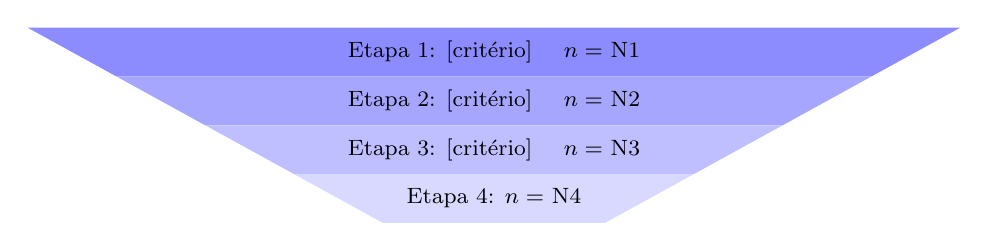
\begin{tikzpicture}[x=\columnwidth/8.6, y=0.62cm, font=\footnotesize]
  % pirâmide invertida: cada faixa é um trapézio mais estreito que o de cima
  \def\faixa#1#2#3#4#5{%  #1 nível (0 = topo)  #2 meia-largura em cima  #3 meia-largura embaixo  #4 cor  #5 texto
    \fill[#4] (-#2,-#1) -- (#2,-#1) -- (#3,-#1-1) -- (-#3,-#1-1) -- cycle;
    \node[align=center] at (0,-#1-0.5) {#5};}
  \faixa{0}{4.2}{3.4}{blue!45}{Etapa 1: [critério] \quad $n = $ N1}
  \faixa{1}{3.4}{2.6}{blue!35}{Etapa 2: [critério] \quad $n = $ N2}
  \faixa{2}{2.6}{1.8}{blue!25}{Etapa 3: [critério] \quad $n = $ N3}
  \faixa{3}{1.8}{1.0}{blue!15}{Etapa 4: $n = $ N4}
\end{tikzpicture}
\caption{Refinamento da busca em quatro etapas. [Uma frase sua sobre o que sobra no fim.]}
\label{fig:piramide}
\end{figure}

% --- Parágrafo 3 (~200 palavras): o que os N4 artigos fazem (itens 17–20 do checklist)
[Agrupe os artigos incluídos por forma de uso do fuzzy (dentro da rede, sobre a saída, na agregação...).
Quantos em cada grupo. Exemplos, com as citações.]

% --- Parágrafo 4 (~100 palavras): a lacuna (itens 23–24 do checklist)
[O que nenhum dos incluídos faz e que este artigo faz.]

% --- Opcional, se sobrar espaço: limitações da revisão (item 23c) em 1–2 frases.

% texto antigo desta subsecao (para reaproveitar, se quiser):
% \subsection{Sistemas fuzzy e incerteza de redes}
% Em revisão da literatura sobre lógica fuzzy e incerteza de redes profundas, encontramos três formas de uso: dentro da rede (camadas, pooling ou
% neurônios fuzzy), sobre a saída (regras aplicadas às probabilidades finais) e na agregação de vários modelos (por
% exemplo, com a integral de Choquet). Sistemas de regras fuzzy também já foram usados para explicar redes a partir de valores de
% atribuição~\cite{aghaeipoor2023}. Os modelos
% Takagi--Sugeno~\cite{takagi1985} combinam antecedentes linguísticos com consequentes numéricos. Não encontramos trabalhos que apliquem regras
% fuzzy ao comportamento interno de uma rede já treinada para detectar quando ela erra; é essa lacuna que este artigo ocupa.

% =====================================================================
\section{O Sistema Proposto}

Seja $f$ um classificador treinado com $K$ classes, mantido congelado. Para uma entrada $x$, $f$ responde $\hat y(x)$ com confiança $p(x)$:
no caso binário, $p$ é a saída sigmoide da classe positiva e $\hat y = \mathbf{1}[p \ge \tau]$, com o limiar $\tau$ escolhido na validação
(índice de Youden); no caso multiclasse, $p$ é a maior probabilidade do softmax. Dizemos que a rede alucinou em $x$ quando $\hat y(x) \ne y$, e que a alucinação é \emph{confiante} quando, além disso, $p(x)$ está entre os
maiores valores de confiança da rede. Esse é o caso que nos interessa: quando a rede é treinada com rótulos ruidosos, ela aprende
associações erradas e passa a responder errado com confiança alta, de modo que $p$ deixa de distinguir erro de acerto.
O sistema produz uma pontuação $r(x) \in [0,1]$, o risco de alucinação, em três etapas (leitura da rede, fuzzificação e inferência)
e, a partir dela, classifica cada resposta em uma de três zonas (Seção~\ref{sec:zonas}). Nada na rede é alterado ou retreinado.

\subsection{Etapa 1: leitura da rede}
\label{sec:leitura}

\textit{Como a rede classifica, bloco a bloco.}
Uma rede profunda não decide de uma vez: ela transforma a entrada em uma sequência de representações cada vez mais abstratas. Formalmente,
$f$ é a composição de $B$ blocos seguida de uma cabeça de classificação,
\begin{align}
  f &= h \circ \phi_B \circ \cdots \circ \phi_2 \circ \phi_1, \nonumber\\
  \mathbf{Z}_b(x) &= \phi_b\big(\mathbf{Z}_{b-1}(x)\big), \qquad \mathbf{Z}_0(x) = x,
  \label{eq:blocos}
\end{align}
em que $\mathbf{Z}_b(x) \in \mathbb{R}^{C_b \times H_b \times W_b}$ é o mapa de ativações do bloco $b$, com $C_b$ canais sobre uma grade
espacial $H_b \times W_b$. Os primeiros blocos respondem a bordas, cores e texturas; os intermediários, a padrões; os finais, ao objeto
inteiro. Só a cabeça $h$ transforma a última representação em resposta: no caso binário, $p(x) = \sigma\big(h(\mathbf{Z}_B(x))\big)$, com
$\sigma(t) = 1/(1+e^{-t})$. A Fig.~\ref{fig:blocos} ilustra esse percurso. O número de blocos lidos depende da arquitetura: $B=16$ na ResNet-32 (cada bloco
residual), 13 na VGG-16 (cada convolução), 19 na MobileNetV2, 18 na EfficientNet-B0, 17 na ResNet-50 e 12 no ViT-B/16 (cada camada do
\textit{encoder}). No transformer, $\mathbf{Z}_b$ é uma sequência de \textit{tokens}, e o resumo do Passo~1 abaixo é a média sobre os
\textit{tokens} em vez da média espacial.

\begin{figure*}[t]
\centering
\IfFileExists{figuras/blocos.png}{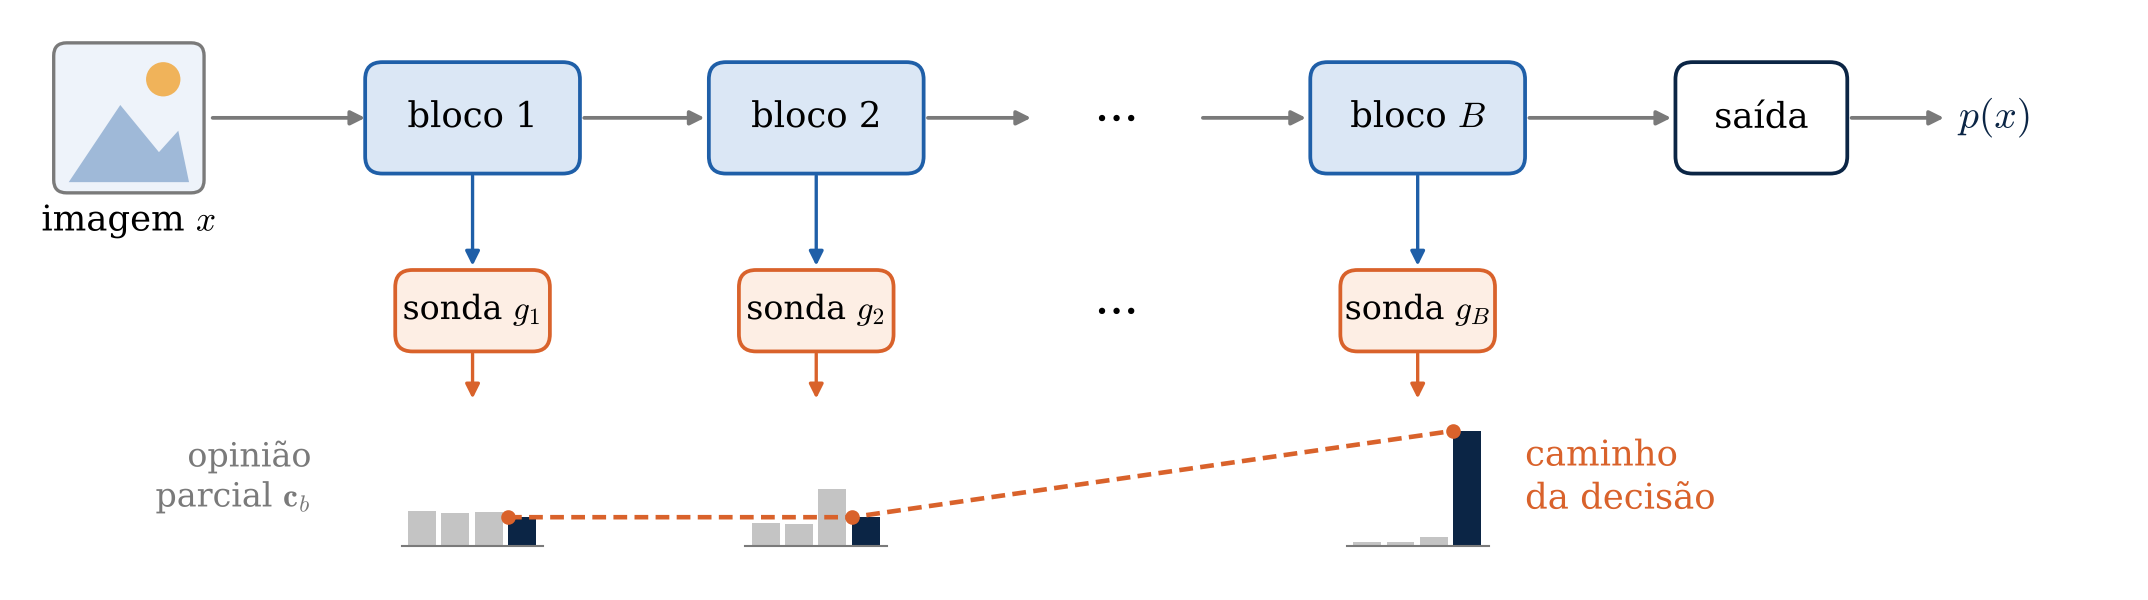
\includegraphics[width=\textwidth]{figuras/blocos.png}}{\fbox{\parbox[c][4.5cm][c]{0.95\textwidth}{\centering
\textcolor{gray}{Espaço reservado para a figura: a imagem passa pelos blocos $\phi_1,\dots,\phi_B$; abaixo de cada bloco, a sonda $g_b$ e
a sua opinião parcial $c_b(x)$. (salvar como figuras/blocos.png)}}}}
\caption{A imagem atravessa os blocos da rede. Em cada bloco, uma sonda lê a representação $\mathbf{a}_b(x)$ e responde o que a rede diria
se parasse ali; a sequência dessas respostas forma o caminho da decisão.}
\label{fig:blocos}
\end{figure*}

\textit{Uma sigmoide em cada bloco.}
Para saber o que a rede ``pensa'' no meio do caminho, colocamos em cada bloco uma sonda linear~\cite{alain2016}. A leitura de um bloco segue
quatro passos.

\emph{Passo 1 (resumo espacial).} O mapa $\mathbf{Z}_b(x)$ é reduzido a um vetor pela média em todas as posições:
\begin{equation}
  \mathbf{a}_b(x) = \frac{1}{H_b W_b} \sum_{u=1}^{H_b}\sum_{v=1}^{W_b} \mathbf{Z}_b(x)_{:,u,v} \in \mathbb{R}^{C_b}.
\end{equation}
Cada coordenada diz o quanto um detector do bloco foi ativado na imagem como um todo.

\emph{Passo 2 (padronização).} Com a média $\mathbf{m}_b$ e o desvio $\mathbf{d}_b$ de cada canal, estimados num conjunto $\mathcal{R}$ de
imagens de referência do treino, e uma projeção $\mathbf{U}_b$ nas 256 componentes principais quando $C_b > 256$,
\begin{equation}
  \tilde{\mathbf{a}}_b(x) = \mathbf{U}_b^{\top}\,\mathrm{diag}(\mathbf{d}_b)^{-1}\big(\mathbf{a}_b(x) - \mathbf{m}_b\big).
\end{equation}

\emph{Passo 3 (a sigmoide do bloco).} A sonda é uma regressão logística sobre $\tilde{\mathbf{a}}_b$. No caso binário,
\begin{equation}
  t_b(x) = \mathbf{w}_b^{\top}\tilde{\mathbf{a}}_b(x) + \beta_b, \qquad c_b(x) = \sigma\big(t_b(x)\big),
  \label{eq:sonda}
\end{equation}
e, com $K$ classes, a sigmoide dá lugar ao softmax,
$g_{b,k}(x) = e^{t_{b,k}(x)}/\sum_{k'} e^{t_{b,k'}(x)}$, com $c_b(x) = g_{b,\hat y(x)}(x)$. Cada bloco tem, portanto, a sua própria curva
sigmoide, com pesos $\mathbf{w}_b$ e viés $\beta_b$ próprios (Fig.~\ref{fig:sigmoide}a): $t_b$ mede de que lado da fronteira o bloco $b$
coloca a imagem, e $c_b \in (0,1)$ é a probabilidade de esse bloco já dar a resposta final da rede.

\emph{Passo 4 (treino das sondas).} O alvo da sonda é a \emph{decisão da rede} $\hat y$, e não o rótulo verdadeiro, porque queremos medir
quando a rede se decide, e não se ela acerta:
\begin{align}
  (\mathbf{w}_b, \beta_b) &= \arg\min_{\mathbf{w},\beta}\; \mathcal{J}_b(\mathbf{w},\beta), \label{eq:treino_sonda}\\
  \mathcal{J}_b(\mathbf{w},\beta) &= \sum_{x \in \mathcal{R}} \omega_{\hat y(x)}\,
     \ell\big(\hat y(x),\, \sigma(\mathbf{w}^{\top}\tilde{\mathbf{a}}_b(x) + \beta)\big) \nonumber\\
     &\quad + \tfrac{1}{2\lambda}\lVert \mathbf{w} \rVert_2^2, \nonumber
\end{align}
em que $\ell$ é a entropia cruzada, $\omega_k$ equilibra as classes e $\lambda = 0{,}1$ controla a regularização. A rede não é alterada:
as sondas apenas observam.

\begin{figure}[t]
\centering
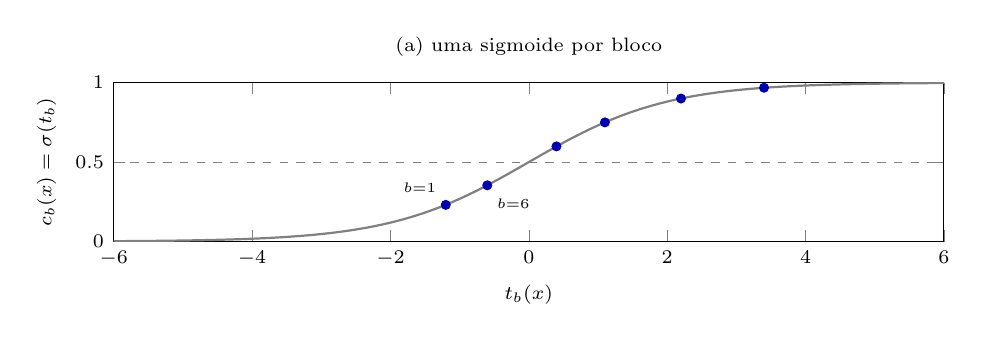
\begin{tikzpicture}
\begin{axis}[width=\columnwidth, height=3.6cm, xmin=-6, xmax=6, ymin=0, ymax=1, xlabel={$t_b(x)$}, ylabel={$c_b(x)=\sigma(t_b)$},
  ylabel style={font=\scriptsize}, xlabel style={font=\scriptsize}, tick label style={font=\scriptsize}, title={(a) uma sigmoide por bloco},
  title style={font=\scriptsize}, ytick={0,0.5,1}, grid=none]
  \addplot[thick, gray, domain=-6:6, samples=100] {1/(1+exp(-x))};
  \addplot[dashed, black!50, domain=-6:6] {0.5};
  \addplot[only marks, mark=*, mark size=1.6pt, blue!70!black] coordinates {(-1.2,0.231) (0.4,0.599) (-0.6,0.354) (1.1,0.750) (2.2,0.900) (3.4,0.968)};
  \node[font=\tiny, anchor=south east] at (axis cs:-1.2,0.25) {$b{=}1$};
  \node[font=\tiny, anchor=north west] at (axis cs:-0.6,0.33) {$b{=}6$};
  \node[font=\tiny, anchor=south east] at (axis cs:3.4,0.97) {$b{=}18$};
\end{axis}
\end{tikzpicture}

\vspace{2pt}
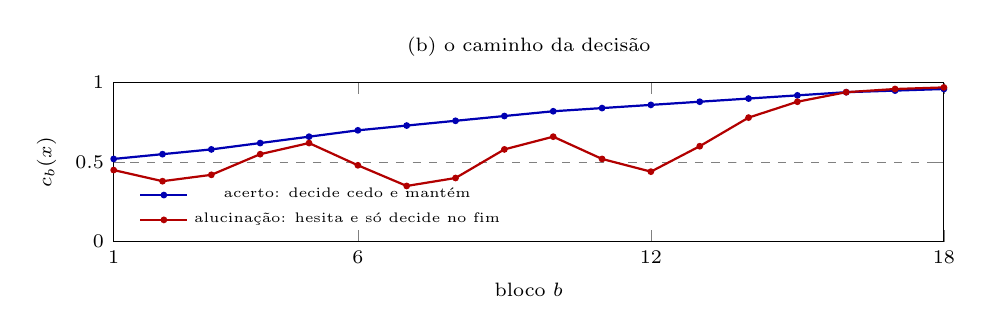
\begin{tikzpicture}
\begin{axis}[width=\columnwidth, height=3.6cm, xmin=1, xmax=18, ymin=0, ymax=1, xlabel={bloco $b$}, ylabel={$c_b(x)$},
  ylabel style={font=\scriptsize}, xlabel style={font=\scriptsize}, tick label style={font=\scriptsize}, title={(b) o caminho da decisão},
  title style={font=\scriptsize}, ytick={0,0.5,1}, xtick={1,6,12,18}, legend style={font=\tiny, at={(0.02,0.02)}, anchor=south west, draw=none, fill=none}]
  \addplot[dashed, black!50, domain=1:18, forget plot] {0.5};
  \addplot[thick, blue!70!black, mark=*, mark size=0.8pt] coordinates {(1,0.52) (2,0.55) (3,0.58) (4,0.62) (5,0.66) (6,0.70) (7,0.73) (8,0.76) (9,0.79) (10,0.82) (11,0.84) (12,0.86) (13,0.88) (14,0.90) (15,0.92) (16,0.94) (17,0.95) (18,0.96)};
  \addlegendentry{acerto: decide cedo e mantém}
  \addplot[thick, red!70!black, mark=*, mark size=0.8pt] coordinates {(1,0.45) (2,0.38) (3,0.42) (4,0.55) (5,0.62) (6,0.48) (7,0.35) (8,0.40) (9,0.58) (10,0.66) (11,0.52) (12,0.44) (13,0.60) (14,0.78) (15,0.88) (16,0.94) (17,0.96) (18,0.97)};
  \addlegendentry{alucinação: hesita e só decide no fim}
\end{axis}
\end{tikzpicture}
\caption{(a) Cada bloco $b$ tem a sua sigmoide (Eq.~\ref{eq:sonda}); os pontos mostram onde uma mesma imagem cai em alguns blocos.
(b) Ligando as respostas de todos os blocos, obtemos o caminho da decisão. Valores ilustrativos.}
\label{fig:sigmoide}
\end{figure}

\textit{Do caminho às características.}
Para cada imagem, as $B$ sigmoides produzem o caminho $\mathbf{c}(x) = \big(c_1(x), \dots, c_B(x)\big) \in [0,1]^B$, em que a posição
$b/B$ é a profundidade relativa. Seja $s_b(x) = \mathbf{1}\big[\arg\max_k g_{b,k}(x) = \hat y(x)\big]$ o indicador de que o bloco $b$ já
concorda com a resposta final (no caso binário, $s_b = \mathbf{1}[c_b > 1/2]$). Resumimos o caminho por cinco funcionais, cada um ligado
a um comportamento da rede:
\begin{align}
  \mathrm{TV}(x) &= \sum_{b=2}^{B} \big| s_b(x) - s_{b-1}(x) \big| \nonumber\\
     &= \sum_{b=2}^{B} \mathbf{1}\big[(c_b - \tfrac12)(c_{b-1} - \tfrac12) < 0\big], \label{eq:tv}\\
  D(x) &= \frac{1}{B}\,\max\big(\{0\} \cup \{\, b : s_b(x) = 0 \,\}\big), \label{eq:prof}\\
  \bar H(x) &= \frac{1}{B\log K} \sum_{b=1}^{B} \Big( -\sum_{k=1}^{K} g_{b,k}(x)\log g_{b,k}(x) \Big), \label{eq:ent}\\
  A(x) &= \frac{1}{|\mathcal{L}|} \sum_{b \in \mathcal{L}} c_b(x), \label{eq:conc}\\
  J(x) &= \big|\, p_{\hat y}(x) - c_B(x) \,\big|. \label{eq:salto}
\end{align}
A \emph{variação total} $\mathrm{TV}$ (Eq.~\ref{eq:tv}) conta quantas vezes o caminho cruza a fronteira $c_b = 1/2$, isto é, quantas vezes
a rede muda de opinião; no binário, a segunda forma deixa isso explícito. A \emph{profundidade da decisão} $D$ (Eq.~\ref{eq:prof}) é a
fração da rede percorrida até o último bloco que ainda discordava; vale 0 quando todos os blocos concordam e segue a profundidade de
predição de Baldock et al.~\cite{baldock2021}. A \emph{entropia média das sondas} $\bar H$ (Eq.~\ref{eq:ent}), normalizada para $[0,1]$,
mede o quanto os blocos ficaram indecisos ao longo do caminho, mesmo sem cruzar a fronteira. A \emph{concordância final} $A$
(Eq.~\ref{eq:conc}) é a média do último terço do caminho, $\mathcal{L} = \{B - \lfloor B/3 \rfloor + 1, \dots, B\}$: se a rede responde com confiança mas o fim do caminho não concorda, há algo
errado. Por fim, o \emph{salto final} $J$ (Eq.~\ref{eq:salto}) compara a confiança da cabeça, $p_{\hat y}$, com a do último bloco; um salto
grande indica que a certeza apareceu só na cabeça. Na Fig.~\ref{fig:sigmoide}b, a alucinação tem $\mathrm{TV}=5$ e $D=12/18$, enquanto o acerto tem
$\mathrm{TV}=0$ e $D=0$; as duas terminam com $A$ e $p$ altos, e é só o caminho que revela a hesitação.

\textit{Estabilidade.}
Sejam $T_1 = \mathrm{id}, T_2, \dots, T_V$ transformações que preservam o rótulo (espelhamentos e rotação de 180$^\circ$ em imagens sem
orientação, como lesões de pele; espelhamento horizontal e deslocamentos de 2 pixels no CIFAR; só pequenos deslocamentos no SVHN e no MNIST,
em que espelhar muda o dígito). Medimos o quanto a resposta e o caminho mudam entre essas vistas:
\begin{align}
  \Delta_V(x) &= \frac{1}{V-1}\sum_{v=2}^{V} \mathbf{1}\big[\hat y(T_v x) \ne \hat y(x)\big], \\
  \sigma_V(x) &= \operatorname{std}_{v}\; p_{\hat y(x)}(T_v x), \\
  \sigma_{\mathbf c}(x) &= \frac{1}{B}\sum_{b=1}^{B} \operatorname{std}_{v}\; c_b(T_v x).
\end{align}

\textit{Familiaridade.}
Seja $\mathbf{e}(x)$ a representação da penúltima camada, centrada e normalizada, e $\mathcal{N}_k(x)$ as $k=15$ imagens de referência com
maior similaridade de cosseno $\langle \mathbf{e}(x), \mathbf{e}(x') \rangle$. Medimos se os vizinhos receberam outra resposta e o quanto
estão longe, em relação à distância típica $\bar\delta$ (a mediana da mesma medida entre as próprias imagens de referência):
\begin{align}
  \nu(x) &= \frac{1}{k}\sum_{x' \in \mathcal{N}_k(x)} \mathbf{1}\big[\hat y(x') \ne \hat y(x)\big], \\
  \delta(x) &= \frac{1}{k\,\bar\delta}\sum_{x' \in \mathcal{N}_k(x)} \big(1 - \langle \mathbf{e}(x), \mathbf{e}(x') \rangle\big).
\end{align}

Com o próprio $p$, são onze características candidatas: $p$, $\mathrm{TV}$, $D$, $\bar H$, $A$, $J$, $\Delta_V$, $\sigma_V$, $\sigma_{\mathbf c}$,
$\nu$ e $\delta$. As três de estabilidade exigem $V$ passagens pela rede; as outras, uma.

\emph{Seleção das características.} Testamos as onze, mas o sistema usa apenas quatro: $p$ e mais três.
O motivo é a redundância. Várias candidatas medem quase a mesma coisa: $\mathrm{TV}$ e $D$ contam,
de formas diferentes, a mesma hesitação ao longo dos blocos; $\bar H$ e $\sigma_{\mathbf c}$ sobem juntas;
$J$ e $A$ acompanham de perto a própria confiança $p$. Nos nossos experimentos, essas correlações de
postos chegaram a $|\rho| \approx 0{,}8$ a $0{,}9$ (Tabela~\ref{tab:features}). Colocar características redundantes
no mesmo modelo não traz informação nova, só dobra o número de regras e torna os pesos instáveis
e difíceis de interpretar.

A escolha é feita em dois passos, apenas nos dados de treino de cada dobra. Primeiro, medimos o que
cada característica $f$ acrescenta \emph{além de} $p$: dividimos as imagens em cinco faixas $q$ de $p$ parecido
(quintis) e calculamos a AUROC de $f$ dentro de cada faixa,
\begin{equation}
  \mathcal{U}_{|p}(f) = \sum_{q=1}^{5} \frac{n_q}{n}\,\max\!\big(\mathcal{U}_q(f),\, 1 - \mathcal{U}_q(f)\big),
  \label{eq:auroc_alem}
\end{equation}
em que $\mathcal{U}_q(f)$ é a AUROC de $f$ na faixa $q$ e $n_q$ o número de imagens nela. Dentro de uma faixa, todas
as imagens têm quase a mesma confiança; assim, uma característica que só repete $p$ fica com $\mathcal{U}_{|p} \approx 0{,}5$.
Segundo, partimos de $\mathcal{S} = \{p\}$ e percorremos as candidatas em ordem decrescente de
$\mathcal{U}_{|p}$, aceitando $f$ somente se
\begin{equation}
  |\rho_{\mathrm{S}}(f, g)| < 0{,}85 \quad \text{para toda } g \in \mathcal{S} \setminus \{p\},
  \label{eq:selecao}
\end{equation}
em que $\rho_{\mathrm{S}}$ é a correlação de Spearman, até que $|\mathcal{S}| = 4$. Ficamos em quatro porque,
com três termos por característica, já são doze regras: o bastante para cobrir as três famílias de sinais
(caminho, estabilidade e familiaridade) e ainda pouco para que cada regra seja lida e conferida à mão.
A escolha é refeita em cada dobra de treino. Também relatamos uma variante sem as características de estabilidade,
que exige uma única passagem pela rede.

\begin{table}[t]
\centering
\caption{As onze características candidatas. $|\rho_p|$: mediana da correlação de Spearman com $p$;
Esc.: porcentagem das partições de treino em que a característica foi escolhida
(CIFAR-10 e CIFAR-10N, três redes cada; números provisórios, semente 42).}
\label{tab:features}
\footnotesize
\setlength{\tabcolsep}{3pt}
\begin{tabular}{@{}llp{3.1cm}rr@{}}
\toprule
 & Grupo & O que mede & $|\rho_p|$ & Esc. \\
\midrule
$p$ & resposta & confiança final da rede & 1,00 & 100\% \\
$\sigma_V$ & estabilidade & variação de $p$ entre vistas & 0,71 & 78\% \\
$A$ & caminho & confiança no último terço & 0,77 & 64\% \\
$\sigma_{\mathbf c}$ & estabilidade & variação do caminho entre vistas & 0,44 & 44\% \\
$\delta$ & familiaridade & distância aos vizinhos & 0,73 & 30\% \\
$D$ & caminho & bloco em que a decisão firmou & 0,46 & 28\% \\
$\bar H$ & caminho & indecisão média das sondas & 0,44 & 22\% \\
$\nu$ & familiaridade & vizinhos com outra resposta & 0,49 & 20\% \\
$\Delta_V$ & estabilidade & vistas com outra resposta & 0,50 & 12\% \\
$J$ & caminho & salto do último bloco à saída & 0,84 & 2\% \\
$\mathrm{TV}$ & caminho & trocas de opinião & 0,22 & 0\% \\
\bottomrule
\end{tabular}
\end{table}

\subsection{Etapa 2: fuzzificação}
Cada característica escolhida $x_j$ é descrita por três termos linguísticos, \term{baixo}, \term{médio} e \term{alto}, com funções de
pertinência triangulares que formam uma partição forte (somam 1 em todo ponto), com picos nos percentis 5, 50 e 95 de $x_j$ nos dados de
treino do sistema. Para a resposta binária $p$, os picos são fixos em $\{0, \tau, 1\}$, de modo que \term{médio} significa ``em cima do
limiar de decisão''. Os termos dão um significado legível a valores que, isolados, não dizem nada a quem usa o sistema.

\subsection{Etapa 3: regras e inferência}
A base de regras tem uma regra para cada par característica--termo, na forma ``SE $x_j$ é $k$ ENTÃO o log da chance de alucinação muda em
$w_{jk}$''. A inferência soma as regras disparadas, ponderadas pelo grau de pertinência, e transforma o resultado em risco:
\begin{equation}
  r(\mathbf{x}) = \sigma\Big(b + \sum_{j=1}^{d}\sum_{k=1}^{3} w_{jk}\,\mu_{jk}(x_j)\Big),
  \label{eq:aditivo}
\end{equation}
em que $\mu_{jk}$ é a pertinência de $x_j$ no termo $k$ e $\sigma$ é a função logística. Trata-se de um sistema Takagi--Sugeno de ordem
zero~\cite{takagi1985} com antecedentes simples e consequentes somados (um modelo fuzzy aditivo). Os pesos são aprendidos por regressão
logística com regularização $\ell_2$ sobre as pertinências, tendo como alvo a alucinação ($\hat y \ne y$). Com $d=4$ características, a
base tem 12 regras e um viés. Um peso positivo indica que a condição aumenta o risco; o alerta de uma imagem pode ser explicado listando as
regras de maior contribuição $w_{jk}\mu_{jk}(x_j)$.

Escolhemos regras de um único antecedente por dois motivos. Primeiro, cada regra pode ser lida sozinha, sem combinar condições. Segundo,
o número de regras cresce linearmente com o número de características, o que deixa os pesos estáveis mesmo com poucos exemplos de erro.

\subsection{Etapa 4: três zonas}
\label{sec:zonas}
O risco $r(x)$ ordena as respostas, mas uma aplicação precisa de uma decisão: confiar na rede ou mandar a imagem para revisão.
Para isso, dois limiares dividem as respostas em três zonas,
\begin{equation}
  z(x) = \begin{cases}
    \textsc{seguro},  & r(x) < t_s,\\
    \textsc{alarme},  & r(x) > t_a,\\
    \textsc{incerto}, & \text{caso contrário},
  \end{cases}
  \label{eq:zonas}
\end{equation}
escolhidos para que cada zona tenha uma garantia sobre a taxa de erro da rede. Seja $e_+(t)$ o limite superior de 95\% de
Clopper--Pearson~\cite{clopper1934} da taxa de erro entre as imagens com $r < t$, e $e_-(t)$ o limite inferior de 95\% entre as imagens
com $r > t$. Então
\begin{align}
  t_s &= \max\{\, t : e_+(t) \le \alpha_s \,\}, \nonumber\\
  t_a &= \min\{\, t : e_-(t) \ge \alpha_a \,\},
  \label{eq:limiares}
\end{align}
com $\alpha_s$ igual a um terço da taxa de erro da rede (a zona segura deve errar no máximo um terço do que a rede erra) e
$\alpha_a = 0{,}5$ (no alarme, pelo menos metade das respostas está errada). Os limiares são escolhidos apenas nos dados de treino do
sistema, com as notas fora da partição de uma validação cruzada interna de três partições, para que não sejam ajustados às mesmas
notas que avaliam. Quando a rede erra muito, pode ocorrer $t_a < t_s$; nesse caso a zona \textsc{incerto} fica vazia e tudo o que não é
seguro vai para o alarme.

\subsection{Alucinações confiantes}
\label{sec:confiantes}
Para medir o caso que motiva o trabalho, separamos o grupo $\mathcal{G}_q$ das $q$ imagens de teste em que a rede está mais confiante
(as de maior $p$; usamos $q = 25\%$ e $50\%$). Dentro de $\mathcal{G}_q$, $p$ quase não varia e, por isso, quase não informa. Avaliamos
ali duas versões: o sistema geral, treinado em todas as imagens, e uma versão específica, treinada só em $\mathcal{G}_q$ e
\emph{sem} $p$ entre as características (o $p$ apenas define o grupo). A versão específica responde diretamente à pergunta: a rede está
segura; algo dentro dela indica que errou?

% =====================================================================
\section{Configuração Experimental}

\subsection{Dados e redes}
Escolhemos um conjunto de dados por domínio, todos com rótulos de teste confiáveis, e três redes de famílias diferentes em cada um,
para que o resultado não dependa de uma arquitetura.

\emph{CIFAR-10}~\cite{krizhevsky2009} é a referência sem ruído. \emph{CIFAR-10N}~\cite{wei2022} usa \emph{as mesmas} imagens, mas com os
rótulos de treino dados por pessoas na plataforma Amazon Mechanical Turk; usamos o conjunto \textit{worst} (o pior de três anotações),
com 40,2\% dos rótulos de treino errados. Como só os rótulos de treino mudam, o par CIFAR-10/CIFAR-10N isola o efeito do ruído real.
\emph{ANIMAL-10N}~\cite{song2019} tem cinco pares de animais parecidos (por exemplo, gato e lince), coletados em buscas na internet, com
cerca de 8\% de rótulos de treino errados e um teste verificado. \emph{Chaoyang}~\cite{zhu2022} é um problema médico de histopatologia
colorretal com quatro classes, em que os rótulos de treino vêm de patologistas que discordam entre si e o teste contém apenas imagens com
rótulo de consenso. % TODO conferir no artigo dos autores como o treino e o teste foram rotulados

Em todos os casos os erros são medidos contra os rótulos de teste confiáveis: a rede é treinada com o ruído e avaliada sem ele. As redes
pequenas (ResNet-32~\cite{he2016}, VGG-16 com normalização em lote~\cite{simonyan2015} e MobileNetV2~\cite{sandler2018}) são treinadas do
zero por 100 épocas (60 no ANIMAL-10N, cujas imagens têm 64$\times$64) com SGD, momento de Nesterov e redução cosseno do passo. No
Chaoyang, EfficientNet-B0~\cite{tan2019}, ResNet-50~\cite{he2016} e ViT-B/16~\cite{dosovitskiy2021} pré-treinadas no ImageNet são
ajustadas por 15 épocas com AdamW, em imagens de 224$\times$224, usando 10\% do treino para escolher a melhor época. Cada rede é treinada
uma vez por semente e congelada; 5.000 imagens de treino servem de referência para as sondas, os vizinhos e o Mahalanobis.

\subsection{Detectores comparados}
Todos os detectores pontuam as mesmas imagens de teste da mesma rede congelada (pontuação maior = alucinação mais provável).
\emph{Sem treino:} confiança do softmax (MSP) e entropia~\cite{hendrycks2017}, desvio entre vistas (TTA),
MC Dropout com $T=30$ passagens pela cabeça~\cite{gal2016}, Mahalanobis com covariância compartilhada~\cite{lee2018} e Deep $k$NN~\cite{papernot2018}.
\emph{Com treino:} Chen et al.~\cite{chen2019} (sondas treinadas com o rótulo em todos os blocos, as 3 maiores probabilidades de cada sonda, \textit{gradient boosting}),
Font et al.~\cite{font2025}, Gorbett e Blanchard~\cite{gorbett2022} (SVM linear sobre a penúltima camada) e uma versão pós-treino do
ConfidNet~\cite{corbiere2019}.
\emph{Outros sistemas fuzzy:} Barna et al.~\cite{barna2026} (implicação de Goguen entre as duas maiores probabilidades, sem treino),
Aghaeipoor et al.~\cite{aghaeipoor2023} (regras aprendidas sobre estatísticas das atribuições da penúltima camada),
a regressão evidencial ENNreg~\cite{denoeux2023} e o TSK intervalar de tipo 2 com calibração conforme de Msaddi e
Kumbasar~\cite{msaddi2026}. Os dois últimos preveem a confiança na classe verdadeira e recebem \emph{as mesmas} características
escolhidas para o nosso sistema, de modo que a comparação isola o modelo fuzzy, e não a entrada. Todos os detectores com treino, inclusive o sistema fuzzy, usam a mesma validação cruzada estratificada de
5 partições no conjunto de teste e são avaliados nas pontuações fora da partição.

\subsection{Métricas}
A métrica principal é a AUROC para separar alucinações de acertos. Também relatamos a AUPR das alucinações, a FPR com 95\% de TPR, o excesso
de área sob a curva risco--cobertura (E-AURC)~\cite{jaeger2023} e quantas alucinações são encontradas quando 10\%, 20\% e 30\% das entradas
mais suspeitas são encaminhadas a uma pessoa. As diferenças de AUROC são testadas em cada rodada com bootstrap pareado (1.000 reamostragens
comuns a todos os métodos); uma diferença é significativa quando o intervalo de 95\% não contém o zero. Para as zonas, relatamos a fração das imagens em cada uma,
a taxa de erro da rede dentro dela e a fração dos erros que ela captura; para as alucinações confiantes, a AUROC dentro de $\mathcal{G}_q$.

% =====================================================================
\section{Resultados}


\subsection{Detecção de alucinações}
Os resultados mostram a AUROC. O sistema fuzzy tem a maior média em seis dos oito cenários e empata com o softmax no SVHN (0,926);
no MNIST, em que a rede erra em menos de 1\% das imagens, fica 0,004 abaixo do melhor detector. Também tem o menor E-AURC nesses mesmos seis
cenários, por exemplo 14,8 contra 22,0 de Chen et al.\ e 45,4 do MSP no CIFAR-10 com ruído.

Os resultados mostram o resultado central: o ganho sobre a confiança da rede cresce à medida que essa confiança deixa de ser
confiável. É desprezível no MNIST e no SVHN, de 0,01 a 0,02 no CIFAR limpo, de 0,05 a 0,09 no HAM10000 e de 0,11 no CIFAR-10 com ruído nos
rótulos. O ruído é o caso extremo de alucinação: as últimas camadas memorizam rótulos errados e o softmax fica confiante no erro, enquanto
as sondas mostram que os blocos anteriores discordavam. Em relação a Chen et al., o concorrente que também lê as camadas internas, o sistema
fuzzy é significativamente melhor em 18 de 26 rodadas e pior em nenhuma , apesar de usar só 12 regras em vez de um
\textit{gradient boosting} sobre todas as sondas.

No HAM10000 o quadro é mais equilibrado: o sistema fuzzy (0,916), Chen et al.\ (0,909) e o modelo só com a saída (0,907) ficam próximos, e o
ganho sobre Chen et al.\ é significativo em uma de cinco sementes. Encaminhando 20\% das imagens, os três encontram 106, 104 e 107 de cada 139
alucinações por 1.000 imagens , contra 82 do MSP e do MC Dropout. Nesse cenário, a vantagem do sistema fuzzy está
na explicação, não na ordenação.

A variante de uma passagem, sem as características de estabilidade, mantém a maior parte do ganho onde a rede mais alucina (0,896 no CIFAR-10
com ruído e 0,914 no HAM10000), mas no CIFAR-10 limpo a estabilidade é necessária para superar o softmax (0,919 contra 0,928).

\subsection{O que as regras dizem}
As regras aprendidas são curtas e coerentes com a intuição. No CIFAR-10 com ruído (semente 42), as regras dominantes tratam do fim do caminho:
SE a concordância final é \term{baixa} ENTÃO $+1{,}57$ no log da chance de alucinação; SE é \term{alta} ENTÃO $-2{,}18$. No HAM10000
(semente 42), estar em cima do limiar aumenta o risco ($p$ \term{médio}: $+1{,}32$), um salto final \term{baixo} o diminui ($-1{,}53$) e
um desvio do caminho \term{alto} entre vistas o aumenta ($+1{,}16$). Ou seja, o sistema aprende que a rede alucina quando o fim da rede discorda
da resposta, quando a resposta está em cima do limiar ou quando o caminho muda com uma simples transformação da imagem.
Em dez reamostragens bootstrap, a correlação de Spearman entre os pesos das regras fica entre 0,90 e 0,98 nos cenários do CIFAR e entre 0,91 e
0,94 no HAM10000 com todas as lesões: as mesmas regras reaparecem quando os dados mudam. A Fig.~\ref{fig:pertinencias} mostra os termos e os pesos.

\begin{figure}[t]
\centering
\IfFileExists{figuras/pertinencias.png}{\includegraphics[width=\columnwidth]{figuras/pertinencias.png}}{\fbox{\parbox{0.9\columnwidth}{\centering\vspace{1cm}
coloque figuras/pertinencias.png (gerada por mostrar\_pertinencias.py)\vspace{1cm}}}}
\caption{Termos linguísticos (funções de pertinência, acima) e pesos das regras (abaixo) do sistema fuzzy. Um peso positivo aumenta o risco de alucinação.}
\label{fig:pertinencias}
\end{figure}

\subsection{Alucinação e incerteza real}
Verificamos se o risco calculado acompanha incertezas que existem fora do modelo.
\textit{Discordância humana.} No CIFAR-10H~\cite{peterson2019}, com cerca de 50 rótulos humanos por imagem de teste, o sistema fuzzy tem a
maior correlação com a discordância entre as pessoas sob ruído nos rótulos (Spearman de 0,28 contra 0,11 do MSP); nas redes limpas fica acima do
MSP, mas abaixo de Gorbett e Blanchard (0,33 contra 0,37 com a ResNet-32 e 0,30 contra 0,34 com a VGG-16).
\textit{Casos difíceis no HAM10000.} A rede alucina em 29,1\% das lesões que precisaram de biópsia e em 3,1\% das confirmadas sem ela, o que
indica que suas alucinações se concentram nos casos ambíguos também para especialistas.
\textit{Outras fotos do mesmo objeto.} Em lesões fotografadas mais de uma vez, a rede muda de resposta em 21\% delas. Aqui o sistema fuzzy é
menos eficaz (AUROC de 0,63) que a distância ao limiar (0,72): ele foi ajustado para prever alucinações, não instabilidade entre aquisições.

% =====================================================================
\section{Discussão e Limitações}
O sistema fuzzy acrescenta mais quando a saída da rede é menos confiável, que é exatamente quando a alucinação é mais perigosa. Em problemas
fáceis (MNIST, SVHN), a confiança do softmax já está perto do teto e a leitura interna não acrescenta nada; em problemas binários com limiar
bem escolhido, como o HAM10000, a própria saída já é um sinal forte e as regras servem sobretudo para explicar.
O sistema é treinado com as alucinações da rede: com poucos erros, como no subconjunto de 3.000 lesões, a variação entre sementes é grande.
As características de estabilidade multiplicam o custo de inferência por $V$, embora a variante de uma passagem mantenha a maior parte do ganho.
Por fim, o sistema foi treinado e testado na mesma rede; se as regras valem para uma arquitetura que ele nunca viu é uma questão em aberto.

% =====================================================================
\section{Conclusão}
Mostramos que um sistema fuzzy simples, com uma dúzia de regras sobre o comportamento interno da rede, detecta quando uma rede congelada
alucina tão bem quanto os melhores detectores caixa-preta, e melhor que a confiança da própria rede quando essa confiança mais engana.
Cada alerta vem com as regras que o dispararam, o que permite a quem usa a rede entender por que desconfiar dela.
Como trabalho futuro, vamos estudar se as regras se transferem entre arquiteturas e estender o sistema a outras tarefas em que redes alucinam.

% Duplo-cego: sem agradecimentos na submissão.
% \section*{Agradecimentos}

\bibliographystyle{IEEEtran}
\bibliography{refs}

\end{document}
